%
% teil2.tex -- Beispiel-File für teil2 
%
% (c) 2020 Prof Dr Andreas Müller, Hochschule Rapperswil
%
% !TEX root = ../../buch.tex
% !TEX encoding = UTF-8
%
\section{Perfekte geradlinige Bewegung
\label{geradlinig:section:perfekte_geradlinige}}
\kopfrechts{Perfekte geradlinige Bewegung}
Im 19.\,Jahrhundert wurde mathematisch gezeigt, 
dass ein Viergelenkmechanismus keine perfekte geradlinige 
Bewegung erzeugen kann.
Bereits zuvor entwickelte Pierre Frédéric Sarrus einen Mechanismus, 
welcher dieses Problem mit einem Sechsgelenkmechanismus löste.
Dieser Mechanismus ist in Abbildung~\ref{fig:sarrus_link} dargestellt.
Seine Erfindung erhielt jedoch nur wenig Aufmerksamkeit.
Ein möglicher Grund dafür war, dass es sich nicht um einen planaren, 
sondern um einen räumlichen Mechanismus handelte.
Dadurch war die Konstruktion für praktische Anwendungen weniger geeignet.
\begin{figure}[htbp]
    \centering
    \begin{minipage}{0.32\textwidth}
        \centering
        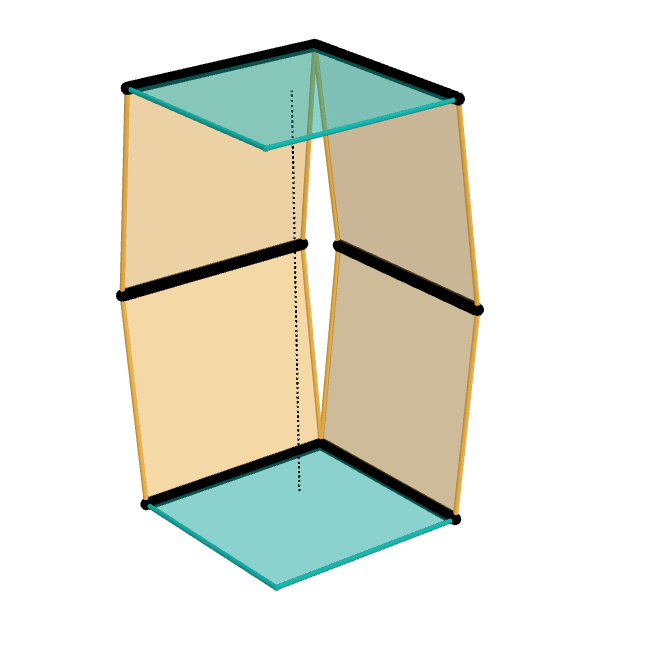
\includegraphics[width=\textwidth]{papers/geradlinig/figures/sarrus_linkage1.png}
    \end{minipage}
    \hfill
    \begin{minipage}{0.32\textwidth}
        \centering
        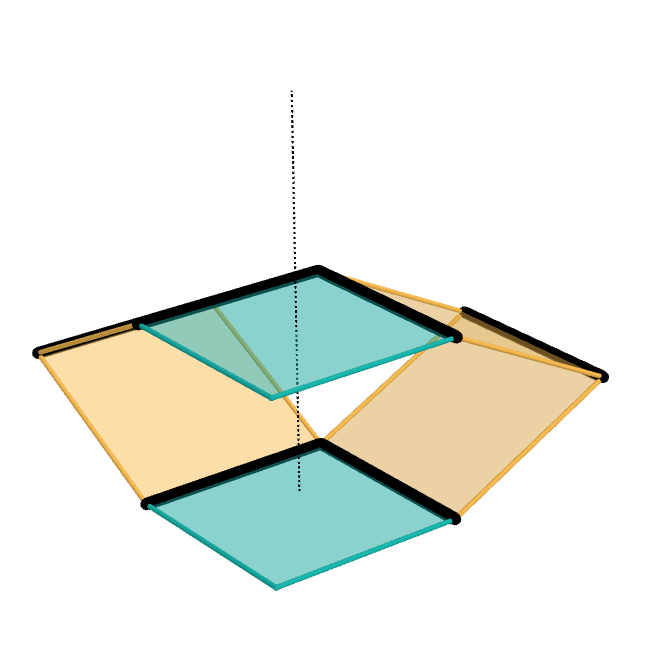
\includegraphics[width=\textwidth]{papers/geradlinig/figures/sarrus_linkage2.png}
    \end{minipage}
    \hfill
    \begin{minipage}{0.32\textwidth}
        \centering
        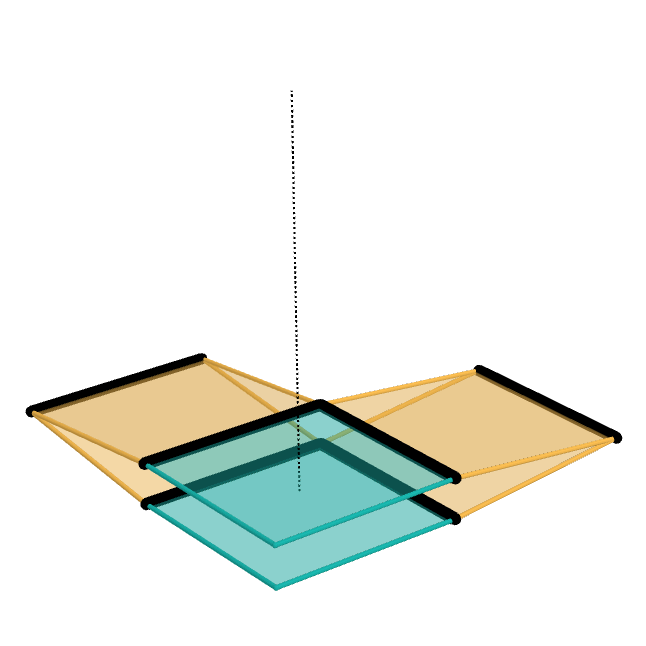
\includegraphics[width=\textwidth]{papers/geradlinig/figures/sarrus_linkage3.png}
    \end{minipage}
    \caption{Der Mechanismus von Sarrus~\cite{sarrus_linkage}.}
    \label{fig:sarrus_link}
\end{figure}

Im Jahr 1864 entwickelte Charles-Nicolas Peaucellier den ersten 
planaren Mechanismus, welcher eine Rotationsbewegung in 
eine perfekte geradlinige Bewegung umwandeln konnte.
Der Mechanismus ist in Abbildung~\ref{fig:peaucellier_link} dargestellt.
Einige Jahre später entwickelte Yom Tov Lipman Lipkin 
unabhängig denselben Mechanismus.
Zu Ehren beider Erfinder wird dieser als 
Peaucellier-Lipkin-Mechanismus bezeichnet.
\begin{figure}[htbp]
    \centering
    \begin{minipage}{0.32\textwidth}
        \centering
        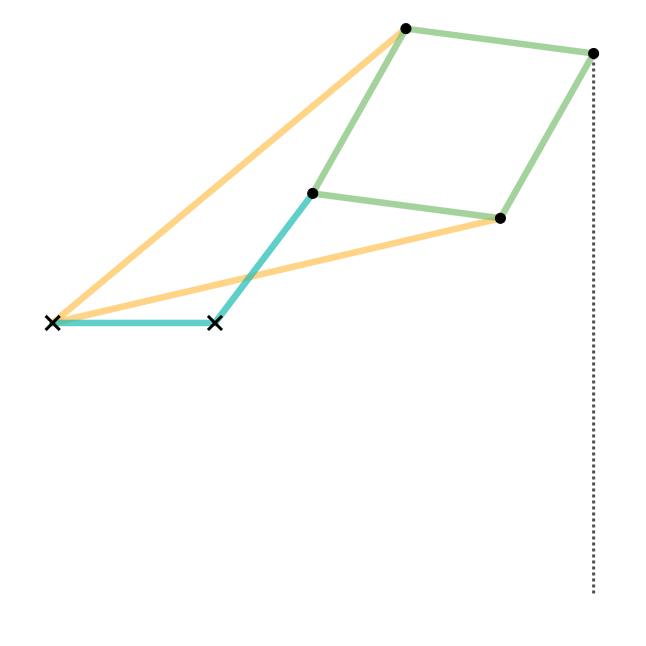
\includegraphics[width=\textwidth]{papers/geradlinig/figures/peaucellier_linkage1.png}
    \end{minipage}
    \hfill
    \begin{minipage}{0.32\textwidth}
        \centering
        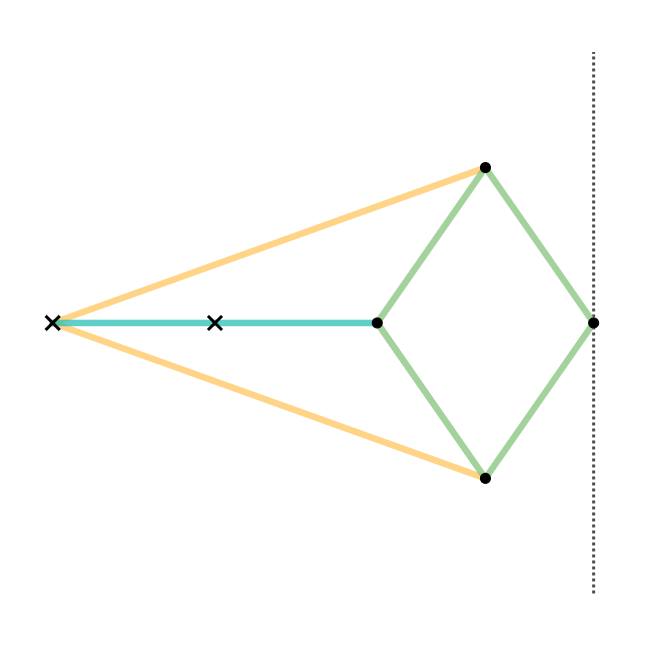
\includegraphics[width=\textwidth]{papers/geradlinig/figures/peaucellier_linkage2.png}
    \end{minipage}
    \hfill
    \begin{minipage}{0.32\textwidth}
        \centering
        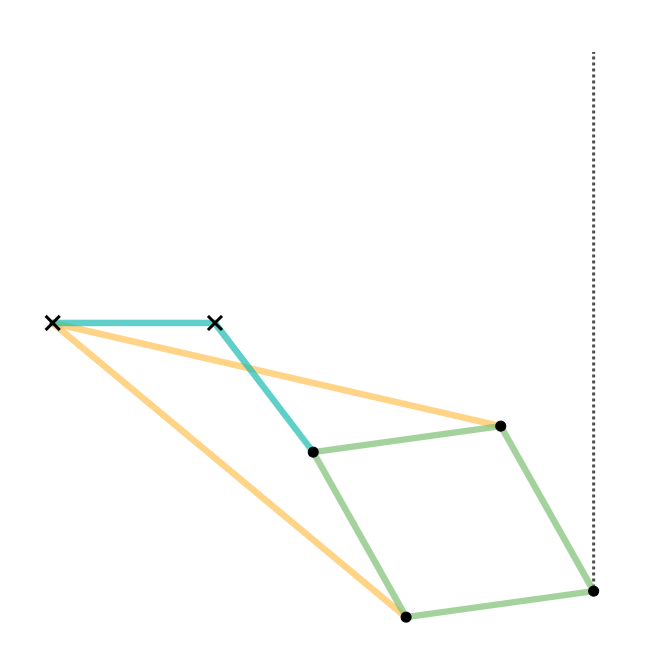
\includegraphics[width=\textwidth]{papers/geradlinig/figures/paucellier_linkage3.png}
    \end{minipage}
    \caption{Der Mechanismus von Peaucellier und Lipkin~\cite{peauc_lip_linkage}.}
    \label{fig:peaucellier_link}
\end{figure}

\subsection{Kreisspiegelung
\label{geradlinig:subsection:geometrische_inversion}}
Die Kreisspiegelung ist eine Transformation der ebenen Geometrie, 
welche das Innere und Äussere eines Kreises vertauscht.
Diese Transformation ist winkeltreu.
Für einen Kreis mit Mittelpunkt $M$ und Radius $R$ wird der Bildpunkt $P'$ 
eines Punktes $P$ dadurch definiert, 
dass $P'$ auf der Geraden $\overline{MP}$ liegt und die Bedingung
\begin{align}
    |\overline{MP'}| |\overline{MP}| = R^2
\end{align}
erfüllt.
Wird anstelle eines einzelnen Punktes eine Gerade gespiegelt, 
entsteht wieder ein Kreis, 
welcher durch den Mittelpunkt $M$ des Inversionskreises verläuft.
Dies ist in Abbildung~\ref{fig:kreisspiegelung} dargestellt.
Die Punkte der ursprünglichen Geraden, welche sich im Unendlichen befinden, 
werden dabei auf den Mittelpunkt $M$ abgebildet.
\begin{figure}[htbp]
    \centering
    \begin{minipage}{0.48\textwidth}
        \centering
        \raisebox{0.1\height}{%
            \input{papers/geradlinig/figures/kreisspiegelung.tex}%
        }
    \end{minipage}
    \hfill
    \begin{minipage}{0.48\textwidth}
        \centering
        \begin{tikzpicture}[scale=2]

  % Circle center M and radius R
  \coordinate (M) at (0,0);
  \def\R{0.8}

  % Circles and Line
  \draw[green, line width=2pt] (M) circle (\R);
  \draw[red, line width=1pt] ($(M)+({\R/2},0)$) circle ({\R/2});
  \draw[blue, thick] ($(M)+(1.2,-1.2)$) -- ($(M)+(1.2,1.2)$);
  \draw[blue, thin, dashed] ($(M)+(1.2,-1.4)$) -- ($(M)+(1.2,1.4)$);

  % Points
  \fill[black] (M) circle (1pt);

  % Labels
  \node[left] at (M) {$M$};

\end{tikzpicture}

    \end{minipage}
    \caption{Illustration der Kreisspiegelung~\cite{kreisspiegelung} an einem Punkt (links) und einer Geraden (rechts).}
    \label{fig:kreisspiegelung}
\end{figure}

Diese Eigenschaft wird beim Peaucellier-Lipkin-Mechanismus verwendet.
Die geometrische Darstellung dieses Mechanismus besteht aus sechs Stäben, 
wie in Abbildung~\ref{fig:geometrie_peauc} dargestellt.
Die Längen $\overline{OA}$ und $\overline{OC}$ sind gleich gross.
Die vier Stäbe $\overline{AB}$, $\overline{BC}$, $\overline{CD}$ und 
$\overline{DA}$ besitzen ebenfalls dieselbe Länge und bilden dadurch eine Raute.
Der Punkt $O$ ist dabei fest im Raum verankert.

Wird der Punkt $B$ auf einer Kreisbahn geführt, 
welche durch den Punkt $O$ verläuft, 
bewegt sich der Punkt $D$ zwingend entlang einer Geraden.
Dies kann beispielsweise durch eine zusätzliche Stange erreicht werden, 
deren Länge der Hälfte der Strecke $\overline{OB}$ entspricht.
Die Kreisbahn von $B$ ist in Rot dargestellt.
Im Gegensatz dazu würde sich Punkt $D$ auf einer Kreisbahn bewegen, 
wenn Punkt $B$ entlang einer Geraden geführt würde, 
welche nicht durch $O$ verläuft.
Auch dieser Kreis würde durch den Punkt $O$ verlaufen.

Es existieren viele verschiedene Proportionen dieses Mechanismus.
Die entscheidende Eigenschaft besteht darin, dass die Punkte $O$, 
$B$ und $D$ während der gesamten Bewegung kollinear bleiben.
Unter dieser Bedingung müssen lediglich die Beziehungen
$\overline{AB} = \overline{AD}$ sowie $\overline{BC} = \overline{DC}$
erfüllt sein.
Zusätzlich muss Punkt $B$ auf einer Kreisbahn geführt werden, 
welche den Punkt $O$ schneidet.
Eine feste Beziehung zwischen den Längen der Seiten des Vierecks $ABCD$ 
ist nicht erforderlich.
\begin{figure}[htbp]
    \centering
    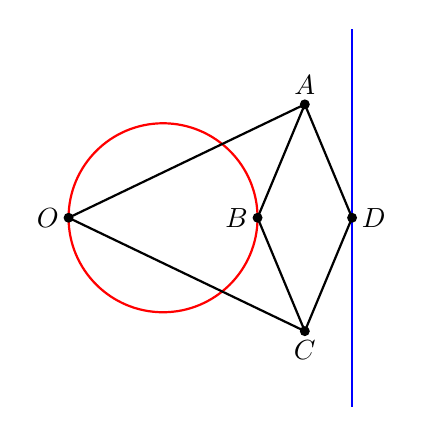
\begin{tikzpicture}[scale=1.2]

  % Circle 
  \def\r{1}
  \draw[red, thick] (0,0) circle (\r);

  % Points on/around circle
  \coordinate (O) at (-\r,0);
  \coordinate (A) at (1.5,1.2);
  \coordinate (C) at (1.5,-1.2);
  
  % Vertical line
  \coordinate (B) at (\r,0);
  \coordinate (D) at (2,0); % 2 = {2*(A.x) - (B.x)}
  \draw[blue, thick] (2,-2) -- (2,2);

  % Quadrilateral OABC
  \draw[thick] (O) -- (A) -- (B) -- (C) -- cycle;

  % Connection to D (diamond-like shape)
  \draw[thick] (A) -- (D) -- (C);

  % Mark points
  \fill (O) circle (1.5pt);
  \fill (A) circle (1.5pt);
  \fill (B) circle (1.5pt);
  \fill (C) circle (1.5pt);
  \fill (D) circle (1.5pt);

  % Labels
  \node[left] at (O) {$O$};
  \node[above] at (A) {$A$};
  \node[left] at (B) {$B$};
  \node[below] at (C) {$C$};
  \node[right] at (D) {$D$};

\end{tikzpicture}

    \caption{Geometrie des Peaucellier-Lipkin-Mechanismus~\cite{peauc_lip_linkage}.}
    \label{fig:geometrie_peauc}
\end{figure}

Ein weiterer Mechanismus inspiriert durch die Kreisspiegelung
ist der Mechanismus von Perrolatz, 
welcher in Abbildung~\ref{fig:perrolatz_link} dargestellt ist.
Dieser besteht ebenfalls aus sechs Stäben.
\begin{figure}[htbp]
    \centering
    \begin{minipage}{0.32\textwidth}
        \centering
        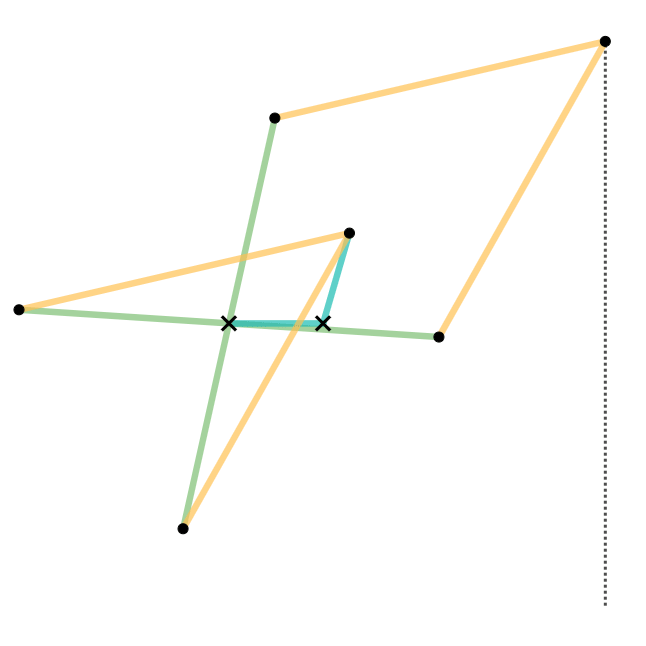
\includegraphics[width=\textwidth]{papers/geradlinig/figures/perrolatz_linkage1.png}
    \end{minipage}
    \hfill
    \begin{minipage}{0.32\textwidth}
        \centering
        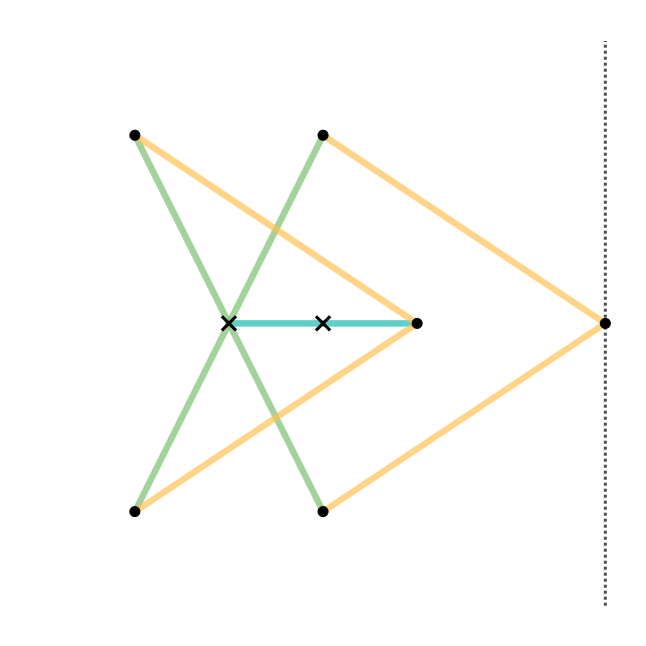
\includegraphics[width=\textwidth]{papers/geradlinig/figures/perrolatz_linkage2.png}
    \end{minipage}
    \hfill
    \begin{minipage}{0.32\textwidth}
        \centering
        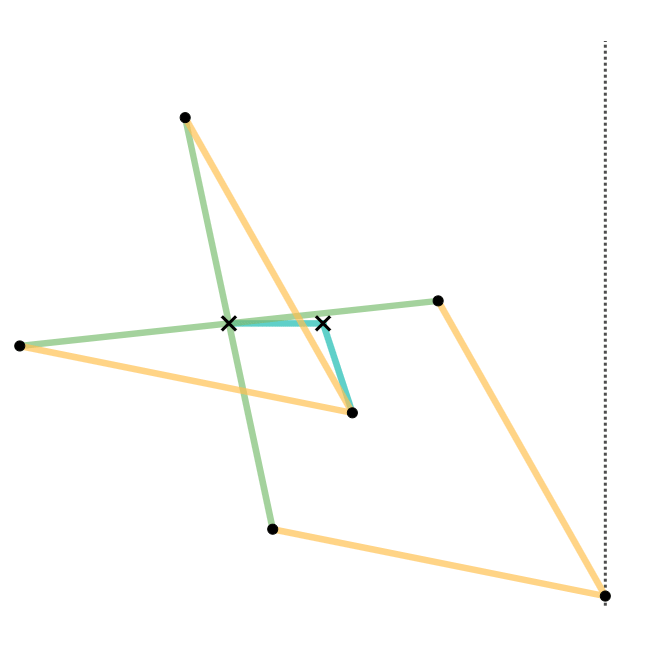
\includegraphics[width=\textwidth]{papers/geradlinig/figures/perrolatz_linkage3.png}
    \end{minipage}
    \caption{Der Mechanismus von Perrolatz~\cite{wiki_straight_line}.}
    \label{fig:perrolatz_link}
\end{figure}

Für diesen Mechanismus gelten die Beziehungen
$\overline{AB}=\overline{CD}$ sowie
$\overline{CQ}=\overline{BQ}=\overline{AP}=\overline{DP}$,
wie in Abbildung~\ref{fig:geometrie_perrolatz} dargestellt.
Der Punkt $E$ bewegt sich dabei auf einer Kreisbahn, während der Punkt $O$ fixiert bleibt.
Dadurch bewegt sich der Punkt $F$ ausschliesslich entlang einer Geraden.
Genau gleich gilt hier auch, dass die Kreisbahn durch $O$ verlaufen muss.
\begin{figure}[htbp]
    \centering
    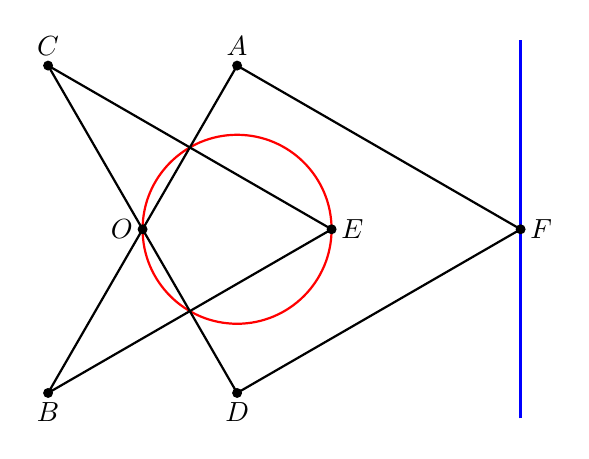
\begin{tikzpicture}[scale=1.2]

  % Foints on/around circle
  \def\len{2}
  \coordinate (A) at ({\len*cos(60)},{\len*sin(60)});
  \coordinate (C) at ({\len*-cos(60)},{\len*sin(60)});
  \coordinate (B) at ({\len*-cos(60)},{\len*-sin(60)});
  \coordinate (D) at ({\len*cos(60)},{\len*-sin(60)});

  % Circle 
  \def\r{1}
  \draw[red, thick] (\r,0) circle (\r);
  
  % Vertical line
  \coordinate (O) at (0,0);
  \coordinate (E) at ({2*\r},0);
  \coordinate (F) at ({2*\r+2*\len*cos(60)},0);
  \draw[blue, thick] ({2*\r+2*\len*cos(60)},-2) -- ({2*\r+2*\len*cos(60)},2);

  % Connections
  \draw[thick] (A) -- (O) -- (B) -- (E) -- (C);
  \draw[thick] (C) -- (D) -- (F) -- (A);

  % Mark points
  \fill (A) circle (1.5pt);
  \fill (B) circle (1.5pt);
  \fill (C) circle (1.5pt);
  \fill (D) circle (1.5pt);
  \fill (F) circle (1.5pt);
  \fill (E) circle (1.5pt);
  \fill (O) circle (1.5pt);

  % Labels
  \node[left] at (O) {$O$};
  \node[right] at (F) {$F$};
  \node[right] at (E) {$E$};
  \node[above] at (A) {$A$};
  \node[below] at (B) {$B$};
  \node[above] at (C) {$C$};
  \node[below] at (D) {$D$};

\end{tikzpicture}

    \caption{Geometrie des Perrolatz-Mechanismus.}
    \label{fig:geometrie_perrolatz}
\end{figure}